
\noindent\begin{minipage}{\textwidth}
    \begin{table}[H]
        \centering
        \caption{Hiperparâmetros e Resultados do Melhor Modelo - swin\_v10\_BR\_opt\_aug}
        \vspace{0.2cm}
        \resizebox{\textwidth}{!}{%
            \begin{tabular}{ll | lrrr}
                \hline
                \multicolumn{2}{c|}{\textbf{Hiperparâmetros}} & \multicolumn{4}{c}{\textbf{Métricas por Classe}} \\ \hline
                \textbf{Parâmetro} & \textbf{Valor} & \textbf{Classe} & \textbf{Precisão} & \textbf{Recall} & \textbf{F1-Score} \\ \hline
    Agendador (Patience) & 6 & 31.2 & 0,6033 & 0,6577 & 0,6293 \\ 
Agendador de LR & ReduceLROnPlateau & 31.3 & 0,4093 & 0,5160 & 0,4565 \\ 
Architecture & swin\_t & 31.4 & 0,4667 & 0,2763 & 0,3471 \\ 
Batch Size & 32 & 32.3 & 0,5978 & 0,5661 & 0,5815 \\ 
Data Augmentation & False & 32.4 & 0,2366 & 0,6111 & 0,3411 \\ 
Decaimento de Peso (WD) & 0,0276 & 33.3 & 0,6720 & 0,3889 & 0,4927 \\ 
Dropout & 0,1011 & 41.4 & 0,2796 & 0,5532 & 0,3714 \\ 
Função de Perda & CrossEntropyLoss & 41.5 & 0,5185 & 0,6512 & 0,5773 \\ 
Hidden Units & 512 & 42.4 & 0,4000 & 0,4262 & 0,4127 \\ 
Label Smoothing & 0,0398 & 44.4 & 0,6667 & 0,8125 & 0,7324 \\ 
\cline{3-6} 
Otimizador & AdamW & \textbf{Média (Macro)} & 0,5017 & 0,5443 & 0,5066 \\ 
Taxa de Aprendizado (LR) & 8,71e-05 & \textbf{MCC} & \multicolumn{3}{c}{0,4279} \\ 
Unfreeze Layers & 1 &  & & &  \\ 
            \hline
            \end{tabular}%
        }
    \end{table}

    \begin{figure}[H]
        \centering
        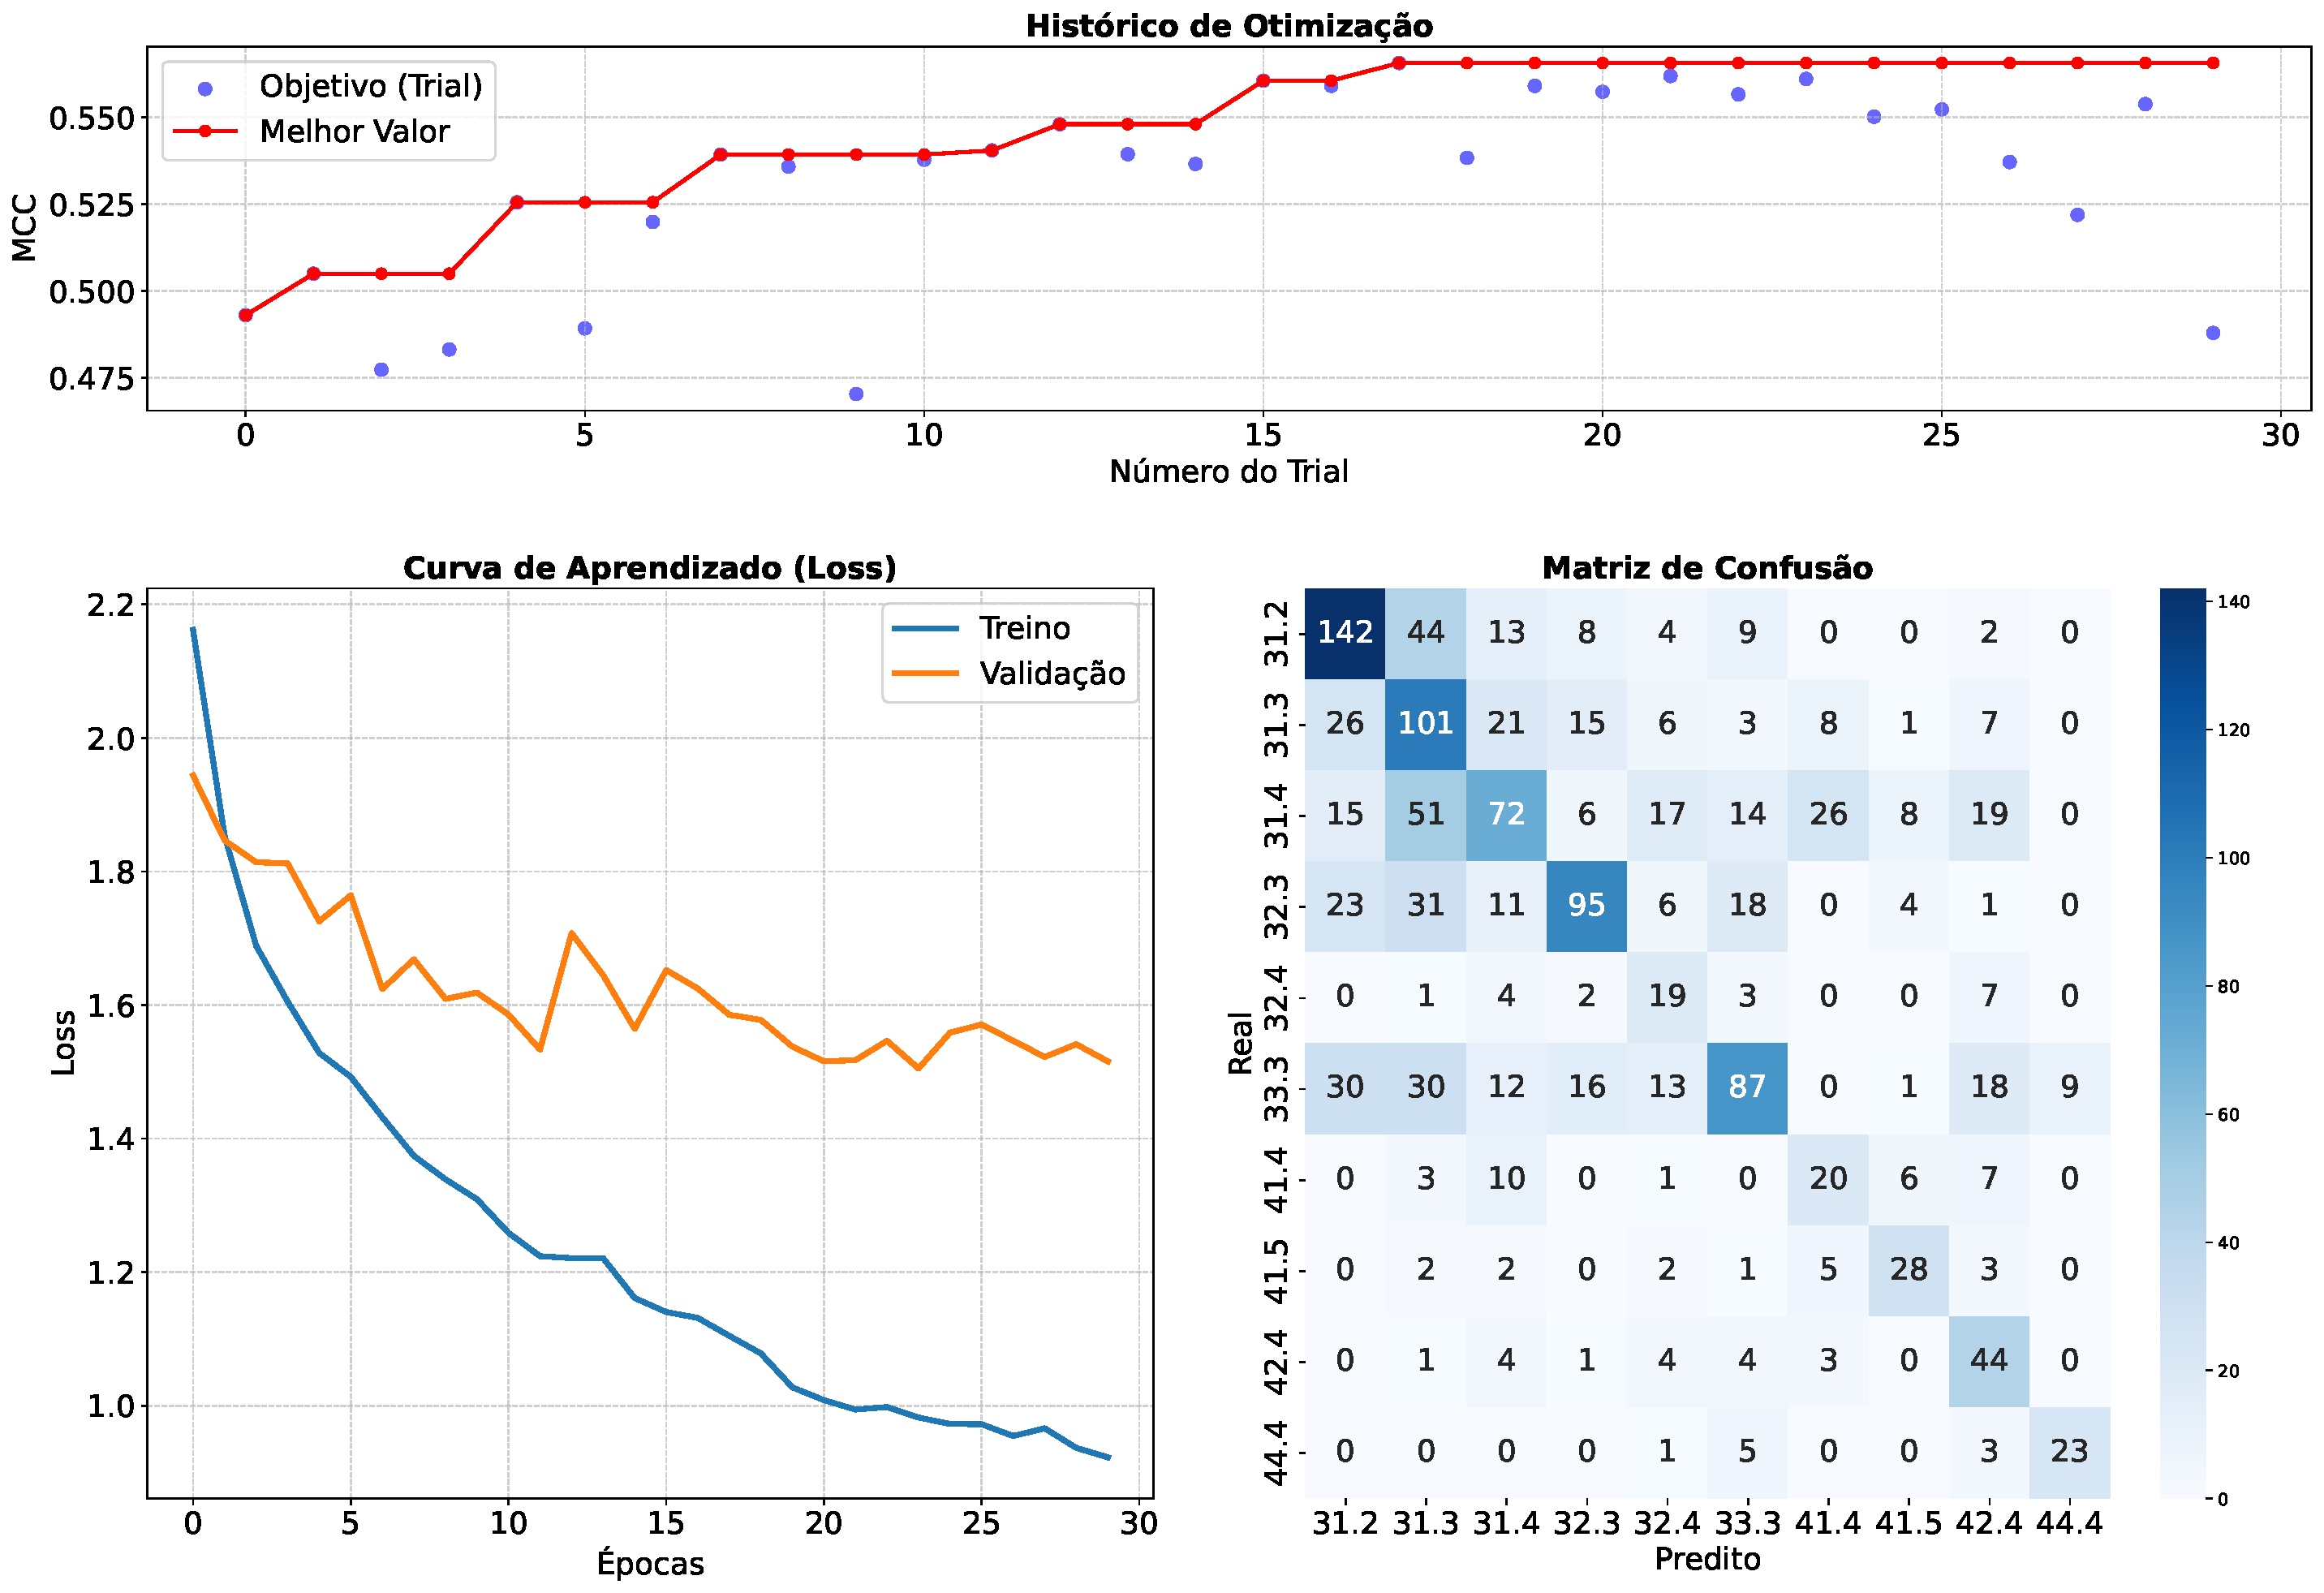
\includegraphics[width=0.85\textwidth]{tex/appendix/experiments/swin_v10_BR_opt_aug/dashboard_consolidado.pdf}
        \caption{Histórico de Otimização, Curvas de Aprendizado e Matriz de Confusão - swin\_v10\_BR\_opt\_aug}
    \end{figure}
\end{minipage}
\clearpage
